\documentclass[a4paper,oneside,12pt]{amsart}

%\usepackage[spanish, activeacute]{babel}
\usepackage[utf8]{inputenc}
%\usepackage[latin1]{inputenc}
\usepackage{latexsym}
\usepackage{multicol}
\usepackage{enumerate}
\usepackage{enumitem}
\usepackage[heightrounded]{geometry}
\geometry{top=2cm,bottom=2cm,left=2cm,right=2cm}
\usepackage{graphicx}
\usepackage{tikz}
\usetikzlibrary{graphs, graphs.standard}
\usepackage{amssymb}
\usepackage{tikz-network}

\DeclareMathOperator{\cond}{cond}
\DeclareMathOperator{\Id}{Id}
\DeclareMathOperator{\re}{Re}
%\DeclareMathOperator{\im}{Im}
\newcommand{\I}{\mathbb{I}}
\newcommand{\R}{\mathbb{R}}
\newcommand{\Q}{\mathbb{Q}}
\newcommand{\C}{\mathbb{C}}
\newcommand{\Z}{\mathbb{Z}}
\newcommand{\N}{\mathbb{N}}
\DeclareMathOperator{\im}{Im}

\newcommand{\nombremateria}
{Investigaci\'on Operativa}
\newcommand{\nombrecuatrimestre}
    {Segundo cuatrimestre de 2025}
\newcommand{\numeroparcial}
    { Tercer Parcial }
\newcommand{\fecha}
    {28 de Noviembre de 2025}
\newcommand{\numerotema}
    {\bf 1}

%\oddsidemargin -1cm \evensidemargin -1cm \textwidth 17.5cm
%topmargin 1.2cm \textheight 25cm
%\setlength{\textheight}{25cm}

\def \ds{\displaystyle}
\theoremstyle{definition}
\newtheorem{quest}{Ejercicio}
\thispagestyle{empty}

\begin{document}

\hfill \hfill
\begin{tabular}[c]{|c|c|c|c|}
\hline 
1 & 2 & 3 & Calificaci\'on \\ \hline \hline
\hspace{1.2 cm} & \hspace{1.2 cm} & \hspace{1.2 cm} &\hspace{1.5 cm} \\
\hspace{1.2 cm} & \hspace{1.2 cm} & \hspace{1.2 cm} &\hspace{1.5 cm} \\ \hline

\end{tabular}

\vspace{-1cm}

\noindent Nombre y apellido:

\vspace{0.2cm}

\noindent Número de libreta:

\noindent \hrulefill 

\smallskip
\renewcommand{\baselinestretch}{1.1}

\begin{center}
	\large \textbf{\nombremateria} 
	
	\numeroparcial -- \fecha
\end{center}

\noindent\textit{Para aprobar el parcial deberá obtenerse un puntaje mayor o igual que 4. \textbf{Entregue todos los ejercicios en hojas separadas.}}

\vspace{.6cm}
\renewcommand{\theenumi}{\textbf{\arabic{enumi}}}

%%% EMPIEZA EL EJERCICIO 1 %%%

\begin{quest}\verb|[3.5 pts.]|
Sea $n \in \mathbb{N}$. El \emph{grafo hipercubo de dimensión $n$}, denotado por $Q_n$, es el grafo simple definido
de la siguiente manera:
\begin{itemize}
    \item El conjunto de vértices es
    \[V_{Q_n} = \{ (a_1, a_2, \ldots, a_n) \mid a_i \in \{0,1\}, \; 1 \le i \le n \} = \{0,1\}^n.\]
    \item Dos vértices $(a_1, a_2, \ldots, a_n)$ y $(b_1, b_2, \ldots, b_n)$ son adyacentes si y sólo si difieren en
    exactamente una coordenada, es decir, existe un único $i \in \{1, \ldots, n\}$ tal que $a_i \ne b_i$.
\end{itemize}
Por ejemplo, $Q_2$ es el siguiente grafo:

\begin{center}
    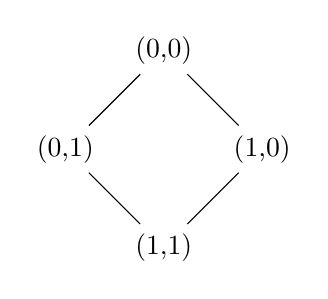
\begin{tikzpicture}
        \node (0) at (0, 1.25) {(0,0)};
        \node (1) at (1.25, 0) {(1,0)};
        \node (2) at (-1.25, 0) {(0,1)};
        \node (3) at (0, -1.25) {(1,1)};

        \draw (0) -- (1) -- (3) -- (2) -- (0);
    \end{tikzpicture}
%\usetikzlibrary {graphs.standard}
%\tikz \graph { subgraph C_n [n=5, clockwise] -> mid };
\end{center}

%\noindent
\begin{enumerate}[label=\alph*)]
    \item \verb|[0.25 pts.]| Calcular la cantidad de aristas de $Q_n$.
    \item \verb|[1 pt.]| Probar que $Q_n$ es un grafo bipartito.
    \item \verb|[1 pt.]| Para cada $v\in V_{Q_n}$ definimos a su padre $p(v)$ como el vértice que se obtiene de
    cambiar a $0$ la
    última coordenada igual a $1$ en $v$. Por ejemplo, en $Q_3$, $p((1,0,1))=(1,0,0)$. Si $v=(0,\dots,0)$, no tiene
    padre. Sea $E=\{(v, p(v))\colon v\neq (0,\dots,0)\}$, probar que $T=(V_{Q_n}, E)$ es un árbol generador de $Q_n$.
    \item \verb|[0.25 pts.]| Probar que $Q_n$ tiene un circuito euleriano si y sólo si $n$ es par.
    \item \verb|[1 pt.]| Probar que $Q_n$ tiene un ciclo hamiltoniano.
%    \item Probar que $Q_n$ es planar si y sólo si $n \le 3$. \\
%    \textbf{Sugerencia:} Demostrar que para todo grafo bipartito, sean $F$ el conjunto de caras, y $E$ el conjunto de aristas
%        $|F| \le \frac{1}{2} |E|$.)
%    \textit
%    {(PISTA: Demostrar que para todo grafo bipartito, sean $F$ el conjunto de caras, y $E$ el conjunto de aristas
%        $|F| \le \frac{1}{2} |E|$.)}

\end{enumerate}
\end{quest}

%%% TERMINA EL EJERCICIO 1 %%%

%%% EMPIEZA EL EJERCICIO 2 %%%


\begin{quest}\verb|[3.5 pts.]|
Sea $G$ el siguiente grafo:

    \begin{center}
        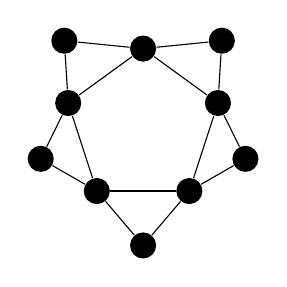
\begin{tikzpicture}
            \graph[nodes={fill=black, circle}, empty nodes, clockwise] { subgraph C_n [V={1,2,3,4,5}, clockwise];
            6[at={(1,1.1)}] -- {1,2};
            7[at={(1.3, -0.4)}] -- {2,3};
            8[at={(0, -1.5)}] -- {3,4};
            9[at={(-1.3, -0.4)}] -- {4,5};
            10[at={(-1, 1.1)}] -- {5,1};
            };

        \end{tikzpicture}
    \end{center}

    \begin{enumerate}[label=\alph*)]
        \item \verb|[0.75 pts.]| Calcular el polinomio cromático de $G$. \\
        \textbf{Sugerencia:} recordar que el polinomio cromático de $C_n$ es $P(k)=(k-1)^n + (-1)^n(k-1)$
        \item \verb|[0.5 pts.]| Calcular el número cromático de $G$.
        \item \verb|[0.75 pts.]| Calcular el índice cromático de $G$.
        \item \verb|[0.5 pts.]| Decimos que un grafo es un grafo perfecto cuando $\omega(H)=\chi(H)$ (es decir,
        cuando el tamaño de la clique
        máxima es igual al número cromático) para cada subgrafo inducido $H$
        del grafo. ¿Es $G$ un grafo perfecto? Justificar.
        \item \verb|[0.5 pts.]|
        Un grafo se dice ``de intervalos" si se pueden representar sus vértices a través de intervalos abiertos
        en la recta real de modo de que cada intervalo está
        asociado a un vértice y dos vertices son adyacentes si y solo si los intervalos se intersecan. Por ejemplo:
        \begin{center}
            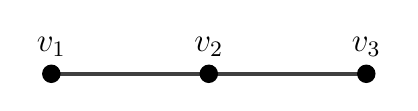
\begin{tikzpicture}
                \SetVertexStyle[FillColor=black, MinSize=0.7]
                \Vertex[label=$v_1$, position=above, fontsize=\large, x=0, y=0]{s1}
                \Vertex[label=$v_2$, position=above, fontsize=\large, x=2, y=0]{s2}
                \Vertex[label=$v_3$, position=above, fontsize=\large, x=4, y=0]{s3}
                \Edge(s1)(s2)
                \Edge(s2)(s3)
            \end{tikzpicture} \hspace{2cm}
            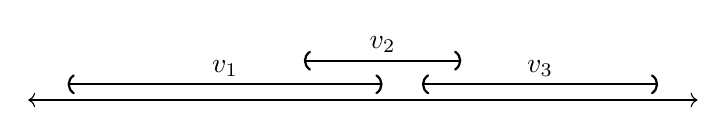
\begin{tikzpicture}
                    \draw[<->] (0,0) -- (8.5,0);
                    \draw[(-), thick] (0.5,0.2) -- (4.5,0.2);
                    \node (v1) at (2.5, 0.4) {$v_1$};

                    \draw[(-), thick] (3.5,0.5) -- (5.5,0.5);
                    \node (v1) at (4.5, 0.7) {$v_2$};

                    \draw[(-), thick] (5,0.2) -- (8,0.2);
                    \node (v1) at (6.5, 0.4) {$v_3$};

                \end{tikzpicture}
        \end{center}
        ¿Es $G$ un grafo de intervalos? Justificar.
        \item \verb|[0.5 pts.]| Un grafo se dice ``arco-circular'' si es el grafo intersección de arcos abiertos
        alrededor de un círculo, es
        decir, si se pueden representar sus vértices a través de dichos arcos de modo de que cada arco está
        asociado a un vértice y dos vertices son adyacentes si y solo si los arcos se intersectan. Por ejemplo:
        \begin{center}
            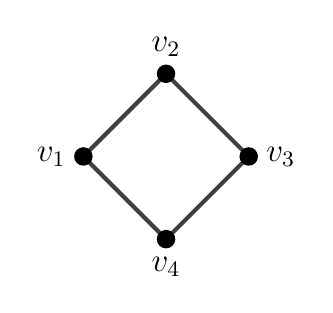
\begin{tikzpicture}[scale=0.7]
                \SetVertexStyle[FillColor=black, MinSize=0.7]
                \Vertex[label=$v_1$, position=left, fontsize=\large, x=0, y=0]{v1}
                \Vertex[label=$v_2$, position=above, fontsize=\large, x=1.5, y=1.5]{v2}
                \Vertex[label=$v_3$, position=right, fontsize=\large, x=3, y=0]{v3}
                \Vertex[label=$v_4$, position=below, fontsize=\large, x=1.5, y=-1.5]{v4}
                \Edge(v1)(v2)
                \Edge(v2)(v3)
                \Edge(v3)(v4)
                \Edge(v4)(v1)
            \end{tikzpicture}\hspace{2cm}
        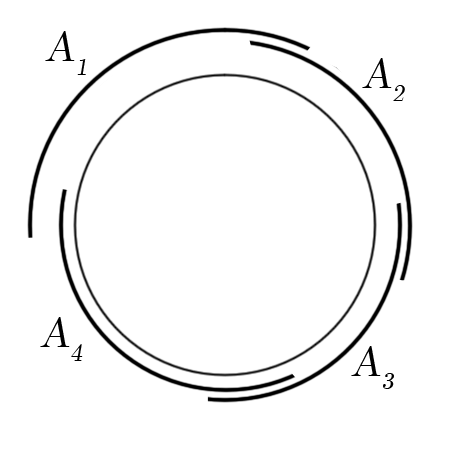
\includegraphics[scale=1]{../2021/Imagenes/arc.png}
        \end{center}
        ¿Es $G$ un grafo arco-circular? Justificar.
%        \item \verb|[0.5 pts.]| Un grafo es círculo si es el grafo intersección de cuerdas dentro de un círculo.
    \end{enumerate}
\end{quest}

%%% TERMINA EL EJERCICIO 2 %%%

%%% EMPIEZA EL EJERCICIO 3 %%%

\begin{quest}
    \verb|[3 pts.]|
    La empresa de turismo Aterrizar.com desea ofrecer un nuevo paquete para viajar desde la ciudad $1$ hasta la
    exótica ciudad $N$. Como la ciudad $N$ está muy lejos de $1$, sólo se pueden llegar haciendo escala en ciudades
    intermedias $2,\dots, N-1$. Se cuenta con un digrafo $G=(V,A)$ que representa las posibles rutas de vuelo: cada
    vértice es
    una ciudad y el arco $(i,j)$ representa que se puede volar de $i$ a $j$. Por simplicidad, podemos suponer que
    si existe el arco $(i,j)$, no existe el arco $(j,i)$ y que $G$ no tiene ciclos. Por ejemplo, un
    mapa de rutas aéreas podría ser el siguiente:
    \begin{center}
        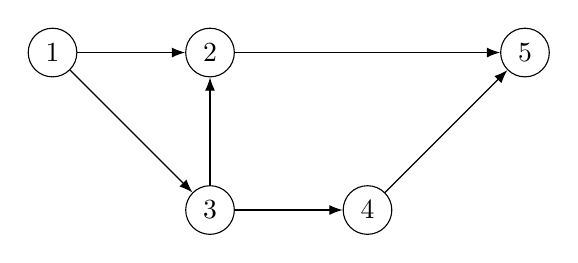
\begin{tikzpicture}
            \node[circle, draw] (1) at (0,0) {1};
            \node[circle, draw] (2) at (2,0) {2};
            \node[circle, draw] (5) at (6,0) {5};
            \node[circle, draw] (3) at (2,-2) {3};
            \node[circle, draw] (4) at (4,-2) {4};

            \draw[-Latex] (1) -> (2);
            \draw[-Latex] (1) -> (3);
            \draw[-Latex] (3) -> (4);
            \draw[-Latex] (3) -> (2);
            \draw[-Latex] (4) -> (5);
            \draw[-Latex] (2) ->  (5);
        \end{tikzpicture}
    \end{center}

    Si $(i, j)\in A$, se conoce el tiempo de vuelo desde $i$ hasta $j$: $t_{ij}$. También, sea $j$ una ciudad y sean
    $i\in N^{-}(j)$,
    $k\in N^{+}(j)$,
    \footnote{$N^{-}(j)=\{k\in V\colon (k,j)\in A\} \quad N^{+}(j)=\{k\in V\colon (j,k)\in A\}$}
    se conoce $escala_{ijk}$,
    el tiempo de escala en $j$ al llegar desde $i$ y esperando el vuelo para partir hacia $k$.
    Naturalmente, en las ciudades $1$ y $N$ no se realiza una escala.
    En el ejemplo, $t_{3,2}=4$ significaría que el vuelo desde $3$ hasta $2$ dura $4$ horas y $escala_{3,2,5}=1$
    significaría que
    la escala en $2$ viniendo desde $3$ y partiendo hacia $5$ tiene una duración de $1$ hora.

    La empresa desea hallar la forma más rápida de llegar desde $1$ a $N$, considerando el tiempo de viaje como
    la suma del tiempo de vuelo y la duración de las escalas. Para un mapa de rutas aéreas $G$,
    modelar el problema como un problema de grafos, proponer un algoritmo para resolverlo en tiempo polinomial y
    calcular cuál es la cantidad de vértices del grafo con el que se modela el problema.
\end{quest}

%%% TERMINA EL EJERCICIO 3 %%%

%%% TERMINA EL PARCIAL %%%



\end{document}

